\documentclass{llncs}
\usepackage{times}
\usepackage[T1]{fontenc}

% Comentar para not MAC Users
%\usepackage[applemac]{inputenc}
\usepackage[utf8]{inputenc}
\usepackage[portuguese]{babel}
\usepackage{a4}
%\usepackage[margin=3cm,nohead]{geometry}
\usepackage{epstopdf}
\usepackage{graphicx}
\usepackage{fancyvrb}
\usepackage{amsmath}
\usepackage{subcaption}
\usepackage{tikz}
\usepackage[bookmarks=false]{hyperref}
\usepackage{float}
%\renewcommand{\baselinestretch}{1.5}

\newcommand{\questionE}[1]{\textcolor{gray}{\textit{"#1"}}}

\begin{document}
\mainmatter
\title{TP3: Camada de Ligação Lógica: Ethernet e Protocolo ARP}

\titlerunning{TP3: Camada de Ligação Lógica: Ethernet e Protocolo ARP}

\author{Sérgio Jorge \and João Freitas \and Alexandre Martins}

\authorrunning{Sérgio Jorge \and João Freitas \and Alexandre Martins}


\institute{
University of Minho, Department of  Informatics, 4710-057 Braga, Portugal\\
e-mail: \{a77730,a74814,a77523\}@alunos.uminho.pt
}

\date{}
\bibliographystyle{splncs}

\maketitle

\section{Introdução}
\hspace{3mm} 

O principal objetivo deste trabalho é o aprofundamento de conhecimentos em redes \textit{Ethernet} e no Protocolo ARP através do estudo e análise de Tramas Ethernet, endereços MAC e tabelas ARP, utilizando ferramentas como \textit{Wireshark} e \textit{CORE}. 

\clearpage

\section{Captura e análise de Tramas Ethernet}

\subsection{Questão 1}
\hspace{3mm} 
\questionE{Anote os endereços MAC de origem e de destino da trama capturada.}\\ 

Como se mostra na figura 1, os endereços são os seguintes:

\begin{itemize}

    \item Origem: \verb|HewlettPdc:ba:3d| com o MAC Address: b0:5a:da:dc:ba:3d
    
    \item Destino \verb|Vmware_5e:69:ad| com o MAC Address: 00:0c:29:5e:69:ad
    
\end{itemize}

\begin{figure}[H]
\begin{center}
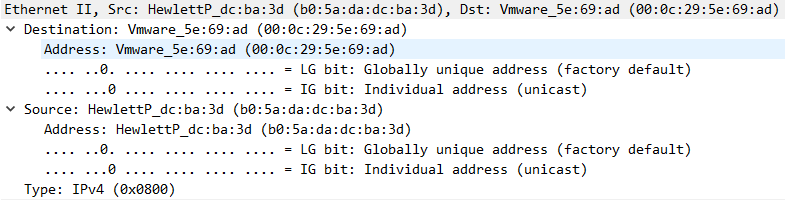
\includegraphics[width=12cm]{1.PNG}
\end{center}
\caption{Endereços MAC envolvidos no HTTP GET}
\end{figure}

\subsection{Questão 2}
\hspace{3mm}
\questionE{Identifique a que sistemas se referem. Justifique.}\\

O endereço MAC origem corresponde à máquina que fez o pedido. Neste caso, refere-se ao computador utilizado para realizar este exercício.

O endereço MAC destino corresponde ao comutador da rede local.

\subsection{Questão 3}
\hspace{3mm}
\questionE{Qual o valor hexadecimal do campo Type da trama Ethernet? O que significa?}\\

O valor do campo é 0x800 e indica o tipo, IPv4.

\begin{figure}[H]
\begin{center}
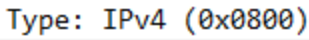
\includegraphics[width=5cm]{3.PNG}
\end{center}
\caption{Campo \textit{type}}
\end{figure}

\clearpage

\subsection{Questão 4}
\hspace{3mm}
\questionE{Quantos bytes são usados desde o início da trama até ao caractere ASCII “G” do método HTTP	GET? Calcule e indique, em percentagem, a sobrecarga (\textit{overhead}) introduzida pela pilha protocolar no envio do HTTP GET.}\\

Desde o início da trama até ao caractere G, são utilizados 53 bytes. Uma vez que o total de bytes da trama é 422, então a percentagem de sobrecarga introduzida pela pilha protocolar é de 12\%.

\begin{figure}[H]
\begin{center}
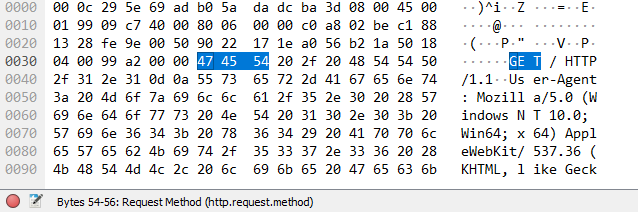
\includegraphics[width=11cm]{4.PNG}
\end{center}
\caption{O caractere G aparece após 53 bytes}
\end{figure}

\subsection{Questão 5}
\hspace{3mm}
\questionE{Através de visualização direta de uma trama capturada, verifique que, possivelmente, o campo FCS (Frame Check Sequence) usado para deteção de erros não está a ser usado. Em sua opinião, porque será?}\\

Nas redes \textit{Ethernet} a utilização de FCS torna-se algo desnecessária por várias razões. Duas delas são a existência de comutadores na rede, que geralmente não enviam pacotes que tenham erros, e também o facto de as redes \textit{Ethernet} se terem tornado muito mais fiáveis e estáveis, o que leva a um número muito reduzido de erros. Por estas e outras razões, não compensa estar a utilizar o campo FCS para cada pacote de informação.

\subsection{Questão 6}
\hspace{3mm}
\questionE{Qual é o endereço Ethernet da fonte? A que sistema de rede corresponde? Justifique.}\\

O endereço Ethernet da fonte é \verb|Vmware_5e:69:ad| (00:0c:29:5e:69:ad). Este endereço corresponde ao comutador da rede local já que, a este nível protocolar, os sistemas só comunicam com máquinas adjacentes a partir do ARP.

\begin{figure}[H]
\begin{center}
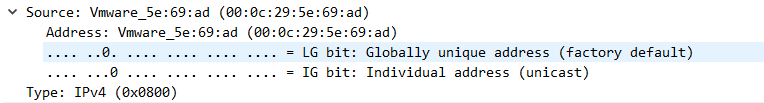
\includegraphics[width=12cm]{6.PNG}
\end{center}
\caption{\textit{Endereço Ethernet fonte de quem fez o HTTP Reply}}
\end{figure}

\clearpage

\subsection{Questão 7}
\hspace{3mm}
\questionE{Qual	é o endereço MAC do destino? A que sistema corresponde?}\\

O endereço MAC do destino é \verb|HewlettP_dc:ba:3d| (b0:5a:da:dc:ba:3d) e corresponde ao computador que foi utilizado para a realização deste exercício. Ou seja, o computador que inicialmente fez o HTTP GET.

\begin{figure}[H]
\begin{center}

\includegraphics[width=12cm]{7.PNG}
\end{center}
\caption{O endereço MAC do destino}
\end{figure}

\subsection{Questão 8}
\hspace{3mm}
\questionE{Atendendo ao conceito de desencapsulamento protocolar, identifique os vários protocolos contidos na trama recebida.}\\

A trama recebida transporta o protocolo \textit{Ethernet 2} no qual está encapsulado o protocolo IPv4, que por sua vez transporta o protocolo TCP, onde está o protocolo HTTP.

\clearpage

\section{Protocolo ARP}

\subsection{Questão 9}
\hspace{3mm} 
\questionE{Observe o conteúdo da tabela ARP. Diga o que significa cada uma das colunas.}\\

Como podemos ver na Figura 6, a tabela ARP é composta por três colunas.
\begin{itemize}
\item{Internet Address} - que indica o endereço IP de uma máquina.
\item{Physical Address} - que indica o endereço MAC de uma máquina.
\item{Type} - que indica se o tipo da ligação entre IP e MAC é estático ou dinâmico.
\end{itemize}

Esta tabela permite manter uma relação entre os endereços IP (\textit{Internet Address}) e MAC (\textit{Physical Address}). A coluna \textit{Type} tem duas opções possíveis, estático ou dinâmico. Uma relação estática significa que esta foi definida manualmente e não se altera. Enquanto que, uma dinâmica é definida no momento em que é estabelecida e fica guardada em cache até que deixe de ser utilizada ou atinja o tempo máximo para ser guardada.  

\begin{figure}[H]
\begin{center}
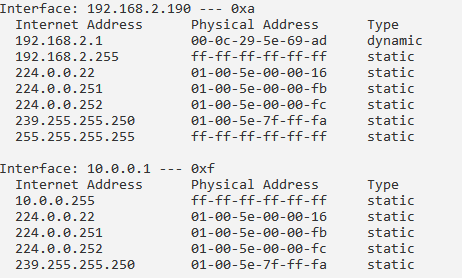
\includegraphics[width=10cm]{9tabelaARP.PNG}
\end{center}
\caption{Tabela ARP}
\end{figure}

\subsection{Questão 10}
\hspace{3mm} 
\questionE{Qual	é o valor hexadecimal dos endereços origem e destino na trama Ethernet que contém a mensagem com o pedido ARP (ARP Request)? Como interpreta e justifica o endereço destino usado?}\\

Como se verifica na figura 7, os endereços são:

\begin{itemize}

    \item Origem: \verb|HewlettPdc:ba:3d| com o MAC Address: b0:5a:da:dc:ba:3d
    
    \item Destino \verb|Broadcast| com o MAC Address: ff:ff:ff:ff:ff:ff
    
\end{itemize}

Neste exercício, o grupo procurou fazer ping a uma máquina de um colega presente na sala de aula. Ou seja, uma vez que, relativamente à máquina destino, só se sabia o endereço IP, então a máquina origem usou o protocolo ARP de forma a descobrir o endereço MAC do destino.

Por isso, é feito o envio de um ARP request para todos os dispositivos na rede local e daí é que surge o \textit{broadcast}. Na figura 8, mostra-se exatamente que o computador usado para a realização do exercício, pergunta à rede quem é o 192.168.2.178 e, mais tarde, essa máquina responde anunciado o seu MAC Address.

\begin{figure}[H]
\begin{center}
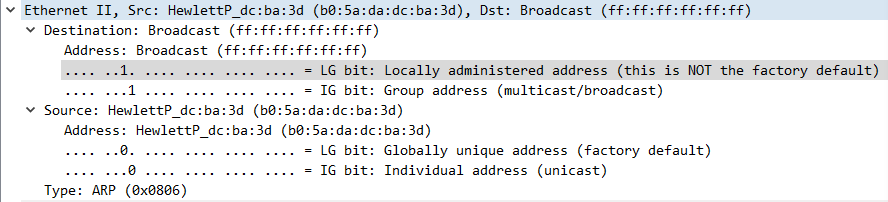
\includegraphics[width=13cm]{10_2.PNG}
\end{center}
\caption{Endereços envolvidos no ARP Request}
\end{figure}

\begin{figure}[H]
\begin{center}
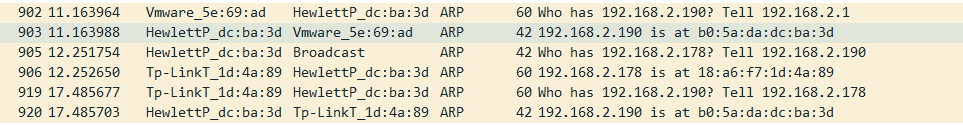
\includegraphics[width=12cm]{10_1.PNG}
\end{center}
\caption{Tramas Ethernet com ARP}
\end{figure}

\subsection{Questão 11}
\hspace{3mm} 
\questionE{Qual o valor hexadecimal do campo tipo da trama Ethernet? O que indica?}\\

O valor do campo é 0x0806 e indica que a trama Ethernet leva ARP encapsulado.

\begin{figure}[H]
\begin{center}
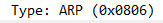
\includegraphics[width=6cm]{11.PNG}
\end{center}
\caption{Tipo da trama Ethernet}
\end{figure}

\clearpage

\subsection{Questão 12}
\hspace{3mm} 
\questionE{Qual	o valor do campo ARP opcode? O que especifica?}\\

Como se mostra na figura 10, o valor do campo opcode é \texttt{request (1)}.

De acordo com a página sugerida, este campo mostra se o ARP é request, que por si só, pode provocar reply a seguir ou se é justamente reply.

Ou seja, prova-se que a trama é um ARP request.

\begin{figure}[H]
\begin{center}
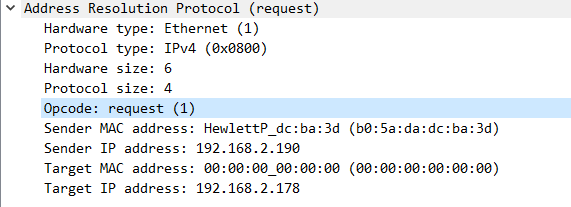
\includegraphics[width=10cm]{12.PNG}
\end{center}
\caption{Protocolo ARP}
\end{figure}

\subsection{Questão 13}
\hspace{3mm} 
\questionE{Identifique que tipo de endereços estão contidos na mensagem ARP? Que conclui?}\\

Os endereços contidos na mensagem ARP são os seguintes:

\begin{itemize}

    \item Sender MAC Address: \verb|HewlettP_dc:ba:3d| (b0:5a:da:dc:ba:3d)
    
    \item Target MAC Address: \verb|00:00:00_00:00:00| (00:00:00:00:00:00)
    
\end{itemize}

Verifica-se, então, que o endereço MAC de destino está a zeros. Significa, por isso, que o endereço destino é desconhecido e que está à espera de ser preenchido.

\begin{figure}[H]
\begin{center}
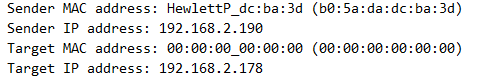
\includegraphics[width=10cm]{13.PNG}
\end{center}
\caption{Endereços na mensagem ARP}
\end{figure}

\subsection{Questão 14}
\hspace{3mm} 
\questionE{Explicite que tipo de pedido ou pergunta é feita pelo host de origem?}\\

Como se mostra na figura seguinte, o computador origem quer saber qual é o endereço MAC da máquina destino, que tem interface com IP 192.168.2.178.

\begin{figure}[H]
\begin{center}

\includegraphics[width=10cm]{14.PNG}
\end{center}
\caption{Descrição do ARP Request}
\end{figure}

\subsection{Questão 15}
\hspace{3mm} 
\questionE{Localize a mensagem ARP que é a resposta ao pedido ARP efectuado.}\\

\subsubsection{15 - A}
\hspace{3mm} 
\questionE{Qual	o valor do campo ARP opcode? O que especifica?}\\

Como se mostra na figura 13, o valor do campo opcode é \texttt{reply (2)}.

De acordo com a página sugerida, este campo mostra se o ARP é request, que por si só, pode provocar reply a seguir ou se é justamente reply.

Ou seja, prova-se que a trama é um ARP reply e que é resposta a um ARP request recebido anteriormente.

\begin{figure}[H]
\begin{center}
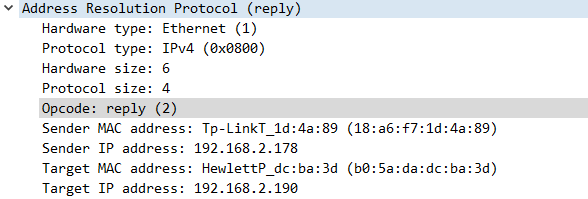
\includegraphics[width=10cm]{15_1.PNG}
\end{center}
\caption{Protocolo ARP}
\end{figure}

\subsubsection{15 - B}
\hspace{3mm} 
\questionE{Em que posição da mensagem ARP está a resposta ao pedido ARP?}\\

A resposta ao pedido ARP está no campo \texttt{Sender MAC Address} onde se especifica que o MAC Address do 192.168.2.178 é o 18:a6:f7:1d:4a:89.

\begin{figure}[H]
\begin{center}
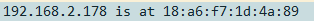
\includegraphics[width=10cm]{15_2.PNG}
\end{center}
\caption{Descrição da resposta}
\end{figure}

\clearpage

\section{ARP Gratuito}

\subsection{Questão 16}
\hspace{3mm} 
\questionE{Identifique um pacote de pedido ARP gratuito originado pelo seu sistema. Analise o conteúdo de um pedido ARP gratuito e identifique em que se distingue dos restantes pedidos ARP. Registe a trama Ethernet correspondente. Qual o resultado esperado face ao pedido ARP gratuito enviado?}\\ 

A seguinte imagem, mostra um ARP request gratuito originado pelo sistema.

\begin{figure}[H]
\begin{center}
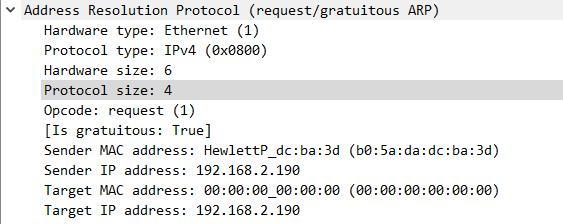
\includegraphics[width=10cm]{16_gratuito_1.PNG}
\end{center}
\caption{ARP gratuito}
\end{figure}

Este tipo de pacote difere dos outros, na medida em que, o IP origem é igual ao IP destino. O pacote irá ser enviado para todas as máquinas na rede local (\textit{broadcast}) e estas vão recebê-lo, atualizando as suas tabelas ARP com o novo endereço IP, em relação aquele MAC.

\begin{figure}[H]
\begin{center}

\includegraphics[width=13cm]{16_gratuito_2.PNG}
\end{center}
\caption{ARP gratuito}
\end{figure}

\clearpage

\section{Domínios de colisão}

\subsection{Questão 17}
\hspace{3mm} 
\questionE{Faça	ping de	n1 para n2.	Verifique com a opção tcpdump como flui o tráfego nas diversas interfaces dos vários dispositivos. Que conclui?}\\

Pela \textit{Figura 17} podemos observar a principal desvantagem de um \textit{Hub}, que é não saber o destino de uma frame e, por isso, manda para todas as interfaces a que está ligado. 
Isto e o facto de um \textit{Hub} ser \textit{Half-Duplex}, o que significa que só uma interface é que pode transmitir de cada vez, faz com que a rede possa ficar sobrelotada aumentando os tempos de resposta e possibilitando colisões.

\begin{figure}[H]
\begin{center}
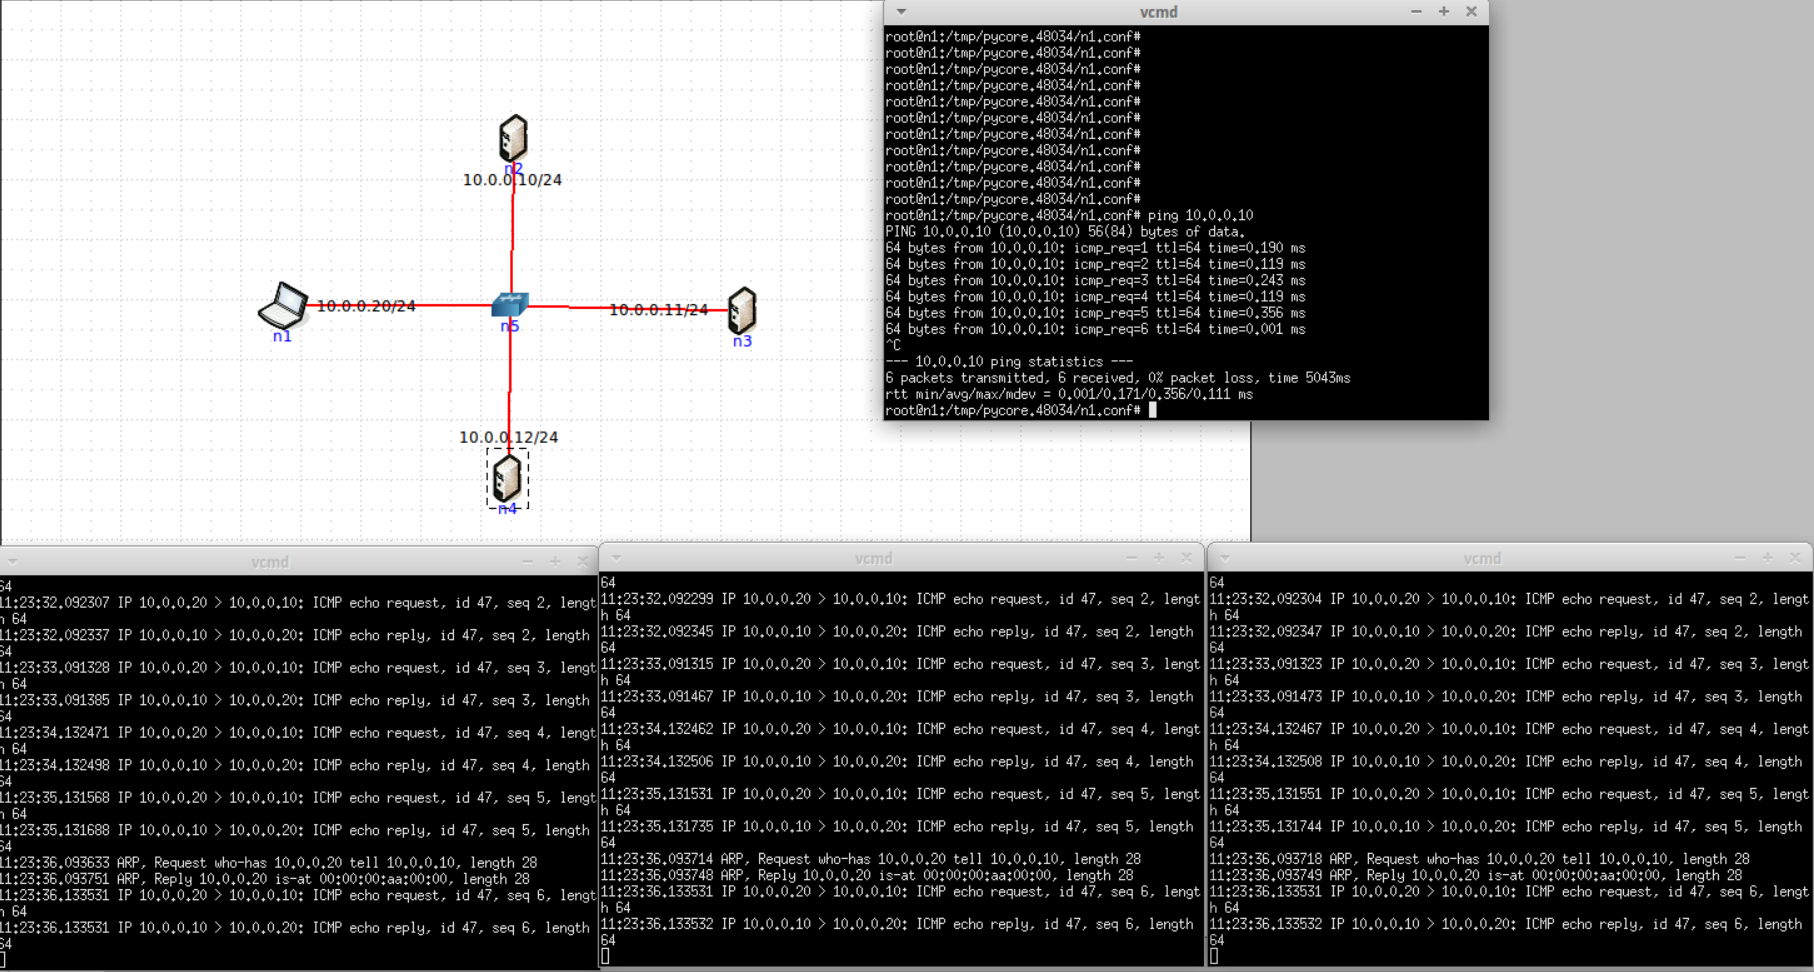
\includegraphics[width=13cm]{ex617.PNG}
\end{center}
\caption{Comando ping do n1 para n2 com Hub}
\end{figure}

\clearpage

\subsection{Questão 18}
\hspace{3mm} 
\questionE{Na topologia de rede substitua o hub por um	switch. Repita os procedimentos que realizou na pergunta anterior. Comente os resultados obtidos quanto à utilização de hubs e switches no contexto de controlar ou dividir domínios de colisão. Documente as suas observações e conclusões com base no tráfego observado/capturado.}\\

Como se pode observar, com o \textit{Switch}, é feito um "ARP Request" a n2, n3 e n4, sendo que só n2 responde com "ARP Reply". 
O \textit{Switch} fica então a saber a interface do n2 logo o "ICMP request" é só feito para n2. 

Os \textit{Switches} têm capacidade de gerir paralelamente os pedidos, logo é impossível haver colisões. 
Como os \textit{Hubs} não têm essa capacidade, existe sempre a possibilidade de haver colisões.

\begin{figure}[H]
\begin{center}
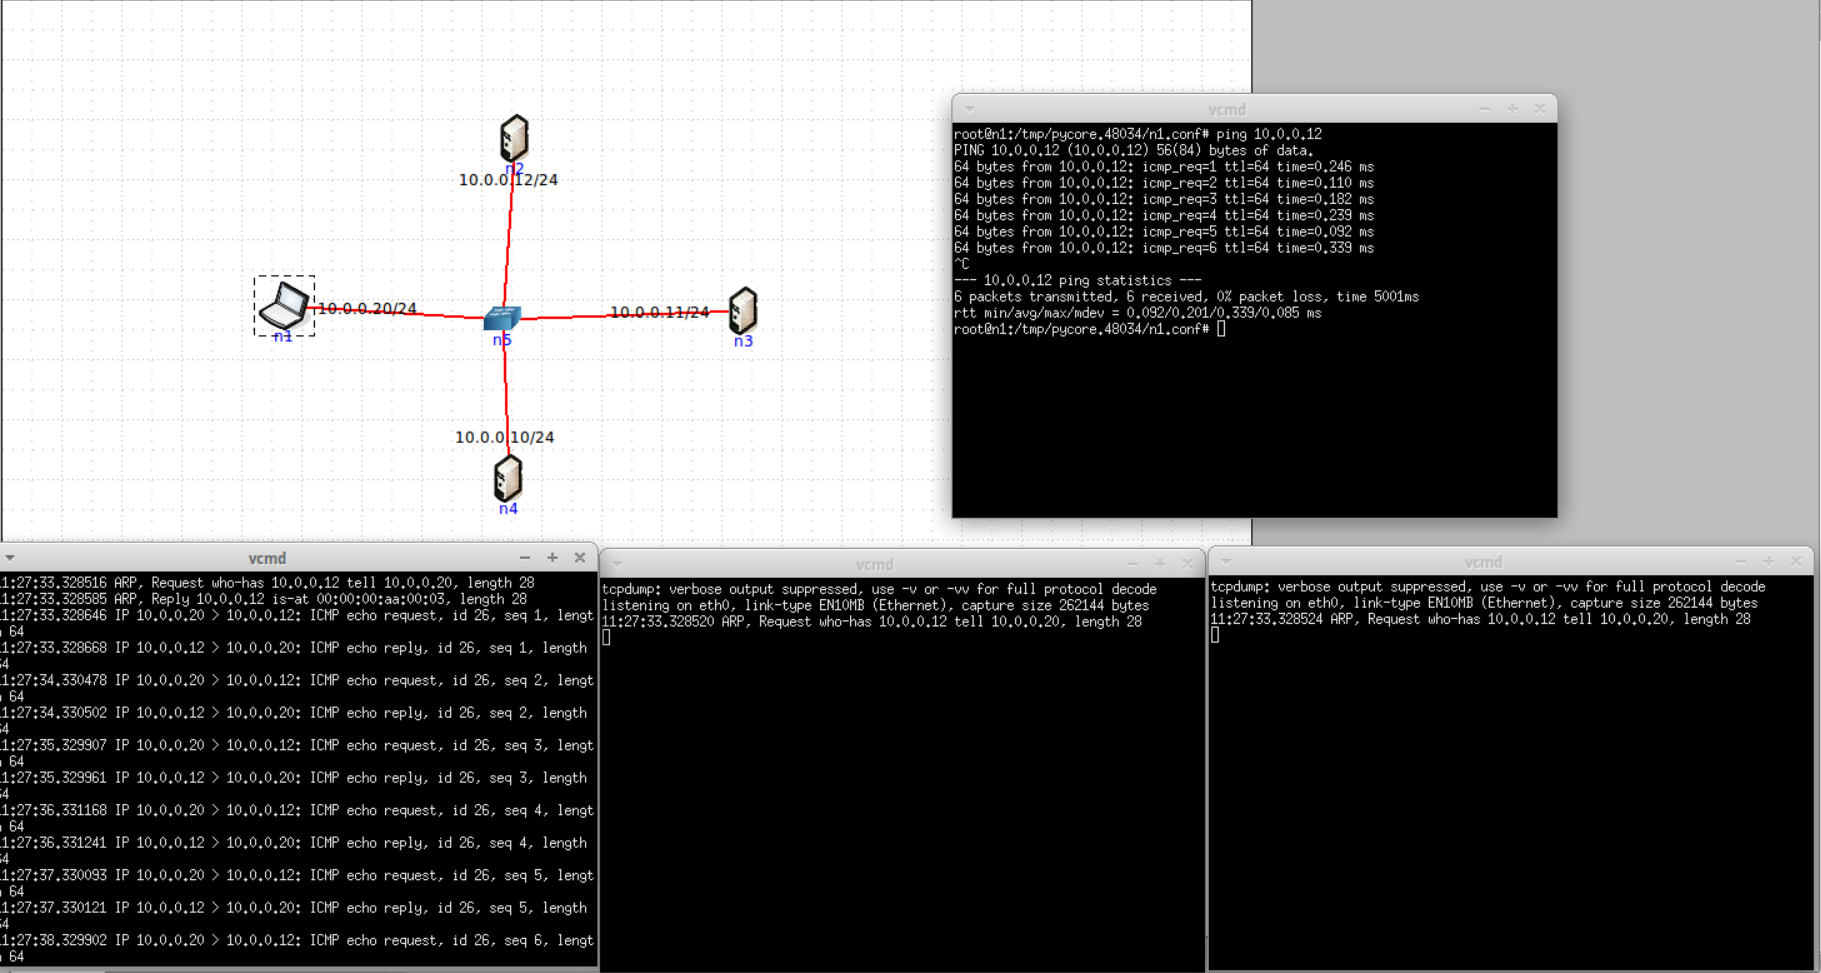
\includegraphics[width=13cm]{ex618.PNG}
\end{center}
\caption{Comando ping do n1 para n2 com Switch}
\end{figure}

\section{Conclusão}
\hspace{3mm}

Neste trabalho, foram analisadas e compreendidas tramas de rede \textit{Ethernet}, o que permitiu ter uma noção mais prática do que acontece na realidade numa rede deste tipo e consolidar bases para uma melhor análise do protocolo ARP.

Através de alguns teste e exemplos conseguiu-se também entender como é que funcionam os endereços MAC e como são atribuídos.

Surgiu, então, o protocolo ARP, e foram analisadas tabelas ARP assim como algumas tramas ARP. Aqui, ficou-se a saber como é feita a relação entre os endereços IP e MAC, utilizando ARP \textit{requests} e \textit{replies}.

Também se estudou as diferenças entre um \textit{Hub} e \textit{Switch} e suas diferenças. Ou seja, os sistemas podem, de facto, ter impacto na rede, principalmente ao nível das colisões e, esses dispositivos dão então perspetivas diferentes do que acontece (uso de diversos protocolos como o CSMA/CD para evitar colisões).

%BIBLIOGRAFIA


\end{document}